%!TEX encoding=UTF-8 Unicode
\documentclass[tikz]{standalone}
\usepackage{tikz}

% Libraries
\usetikzlibrary{shapes,arrows,decorations,decorations.pathreplacing,decorations.markings,fit}
\usetikzlibrary{positioning,backgrounds,calc}

% Layers
\pgfdeclarelayer{background}
\pgfdeclarelayer{bg1}
\pgfdeclarelayer{foreground}
\pgfdeclarelayer{ff}
\pgfsetlayers{background,bg1,main,foreground,ff}
%% Figure: tikz/exp-tikz.tex
\definecolor{envcol}{HTML}{3B8ECC}
\definecolor{distribcol}{HTML}{FF000A}
\definecolor{groupcol}{HTML}{FDAE61}
\definecolor{conceptcol}{HTML}{ABD9E9}
\definecolor{filecol}{HTML}{ABD9E9}

\tikzstyle{env} = [drawed box=envcol, dashed]
\tikzstyle{distrib} = [drawed box=distribcol]
\tikzstyle{group} = [drawed box=groupcol]
\tikzstyle{concept} = [filled box=conceptcol]

\tikzstyle{dep} = [->,filecol,thick]
\tikzstyle{exec} = [->,distribcol,thick]
\tikzstyle{copy} = [->, dashed, thick, groupcol]

\newlength{\cornerlength}
\setlength{\cornerlength}{.145cm}

\tikzset{
  basic box/.style = {
    shape = rectangle,
    draw,
    text centered,
    text width=6em,
    node distance=8em,
    },
  rounded box/.style={
    basic box,
    rounded corners,
  },
  drawed box/.style ={
    rounded box,
    inner sep=1em,
    draw = #1,},
  filled box/.style = {
    rounded box,
    draw  = #1,
    fill  = #1,},
  corner/.style={
      shape=rectangle,
      fill=white,
      alias=this,
      append after command = {
          \pgfextra{
              \begin{pgfonlayer}{ff}
                \draw [black,thin] (this.south west) -- (this.south east);
                \draw [black,thin] (this.south west) -- (this.north west);
                \draw [black,thin] (this.north west) -- (this.south east);
              \end{pgfonlayer}
            }
      }
  },
  file/.style ={
      basic box,
      draw = black,
      fill = filecol,
      minimum height = 5.5em,
      text width = 4em,
      node distance=5em,
      append after command = {
            \pgfextra{\let\TikZlastnode\tikzlastnode}
            node [corner] (corner-TikZlastnode) at
            ([xshift=-\cornerlength,yshift=-\cornerlength]\TikZlastnode.north east){}
          }
  },
  header node/.style = {
    %Minimum Width = header nodes,
    font          = \strut\large,%\ttfamily,
  %  text depth    = +0pt,
    fill          = #1,
    draw},
    header/.style n args={4}{%
    inner ysep = +1.7em,
    append after command = {
      \pgfextra{\let\TikZlastnode\tikzlastnode}
      node [header node=#2,#4] (header-\TikZlastnode) at (\TikZlastnode.#3) {#1}
      %node %[span = (\TikZlastnode)(header-\TikZlastnode)]
       % at (fit bounding box) (h-\TikZlastnode) {}
    }
  },
  hv/.style = {to path = {-|(\tikztotarget)\tikztonodes}},
  vh/.style = {to path = {|-(\tikztotarget)\tikztonodes}},
  fat blue line/.style = {ultra thick, blue}
}
\begin{document}
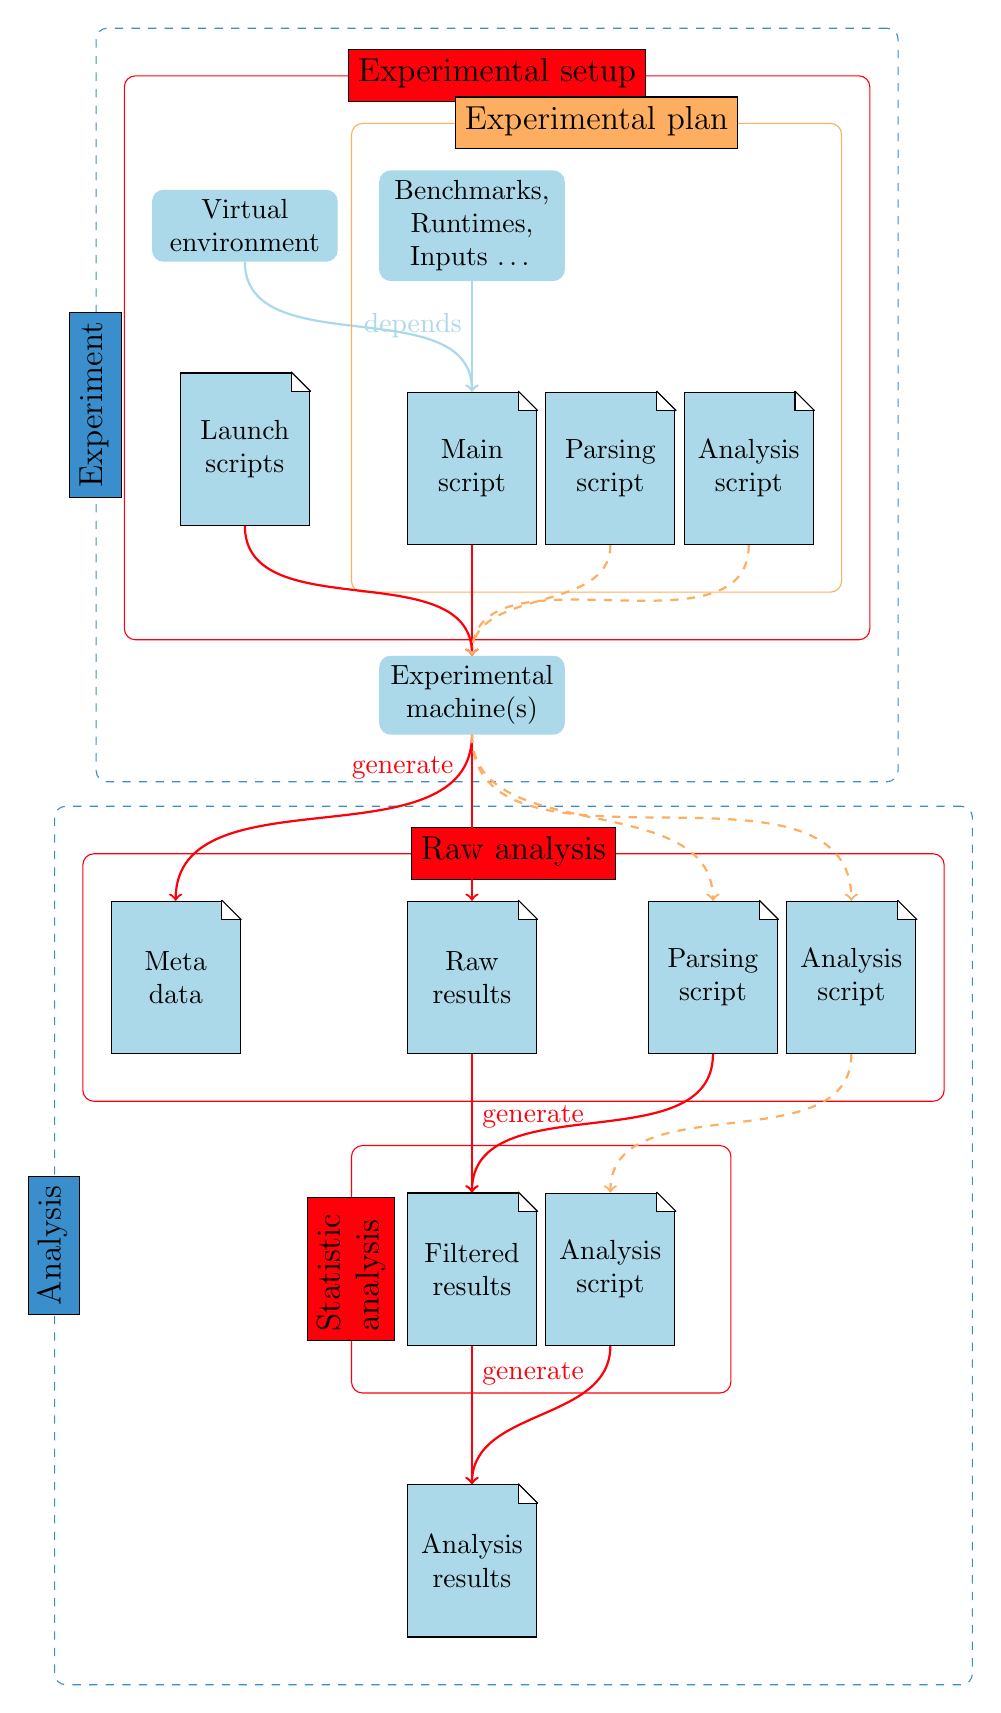
\begin{tikzpicture}[node distance = 2cm,scale=0.8]rotate=90

    %expe env
    \begin{pgfonlayer}{foreground}

    \node [concept] (configs) {Benchmarks, Runtimes, Inputs \ldots};

    \node [concept,left=1.5em of configs] (venv) {Virtual environment};

    \node [file, below=4em of configs] (main) {Main script};
    \node [file, right of=main] (filt) {Parsing script};
    \node [file, right of=filt] (ana) {Analysis script};

    \node [file,below=4em of venv] (dpl) {Launch scripts};

    \node [concept, below= 4em of main] (mach) {Experimental machine(s)};
    \end{pgfonlayer}

    \node [group,fit=(configs) (main) (filt) (ana),header={Experimental plan}
    {groupcol}{north}{}] (plan) {};

    \begin{pgfonlayer}{bg1}
        \node[distrib,fit=(configs) (venv) (plan) (dpl),%
        header={Experimental setup}{distribcol}{north}{}] (distenv) {};
    \end{pgfonlayer}

    \begin{pgfonlayer}{background}
        \node[env,fit=(distenv) (mach),%
        header={Experiment}{envcol}{west}{rotate=90}] (expenv) {};
    \end{pgfonlayer}

    % Analysis env

    \begin{pgfonlayer}{foreground}
        \node[file, below= 6em of mach] (raw) {Raw results};
        \node[file, left= 6em  of raw] (mi) {Meta data};
        \node [file, right= 4em of raw] (filt1) {Parsing script};
        \node [file, right of=filt1] (ana1) {Analysis script};
    \end{pgfonlayer}

    \begin{pgfonlayer}{bg1}
        \node[distrib,fit=(raw) (mi) (filt1) (ana1),%
        header={Raw analysis}{distribcol}{north}{}] (rawa) {};
    \end{pgfonlayer}

    \begin{pgfonlayer}{foreground}
        \node[file, below= 5em  of raw] (csv) {Filtered results};
        \node [file, right of=csv] (ana2) {Analysis script};
    \end{pgfonlayer}

    \begin{pgfonlayer}{bg1}
        \node[distrib,fit=(csv) (ana2),%
        header={Statistic analysis}{distribcol}{west}{rotate=90,text
        width=4.5em}, inner xsep=2em] (stata) {};
    \end{pgfonlayer}

    \begin{pgfonlayer}{foreground}
        \node[file, below= 5em of csv] (res) {Analysis results};
        %\node [concept, right of=res] (com) {Comments};
        %\node [file, below= 3em of res] (pap) {Article};
    \end{pgfonlayer}

    \begin{pgfonlayer}{background}
        \node[env,fit=(rawa) (stata) (res),%
        header={Analysis}{envcol}{west}{rotate=90}] (anaenv) {};
    \end{pgfonlayer}

    % Paths

    \begin{pgfonlayer}{background}
        \path[dep] (configs.south) edge node[left,pos=.4] {depends} (main.north);
        \path[dep] (venv.south) edge[out=270,in=90]  (main.north);
    \end{pgfonlayer}
    % \path[dep] (configs.south) edge[out=270,in=90] node[above] {use} (mach.north);
    \path[exec] (main.south) edge  (mach.north);
     \path[copy] (filt.south) edge[out=270,in=90]  (mach.north);
     \path[exec] (dpl.south) edge[out=270,in=90]  (mach.north);
     \path[copy] (ana.south) edge[out=270,in=90] (mach.north);

    \path[exec] (mach.south) edge[out=270,in=90] node[pos=.1,left] {generate} (mi.north);
    \path[exec] (mach.south) edge[out=270,in=90] (raw.north);
    \path[copy] (mach.south) edge[out=270,in=90] (filt1.north);
    \path[copy] (mach.south) edge[out=270,in=90] (ana1.north);

    \draw[exec] (raw.south) -- node[right,pos=.45] {generate} (csv.north);
    \path[exec] (filt1.south) edge[out=270,in=90] (csv.north);
    \path[copy] (ana1.south) edge[out=270,in=90] (ana2.north);

    \draw[exec] (csv.south) -- node[pos=.2,right] {generate} (res.north);
    \path[exec] (ana2.south) edge[out=270,in=90] (res.north);

    %\draw[exec] (res.south) -- node[left] {generate} (pap.north);
    %\path[exec] (com.south) edge[out=270,in=90] (pap.north);
\end{tikzpicture}
\end{document}
